\documentclass[letterpaper]{article} % DO NOT CHANGE THIS
\usepackage[submission]{aaai2027}  % DO NOT CHANGE THIS
% The serif, sans-serif, and monospaced fonts are loaded automatically by
% aaai2027.sty (newtxtext, helvet, courier). DO NOT add \usepackage{times},
% \usepackage{helvet}, \usepackage{courier}, or any other font package.
\usepackage[hyphens]{url}  % DO NOT CHANGE THIS
\usepackage{graphicx} % DO NOT CHANGE THIS
\urlstyle{rm} % DO NOT CHANGE THIS
\def\UrlFont{\rm}  % DO NOT CHANGE THIS
\usepackage{natbib}  % DO NOT CHANGE THIS AND DO NOT ADD ANY OPTIONS TO IT
\usepackage{caption} % DO NOT CHANGE THIS AND DO NOT ADD ANY OPTIONS TO IT
\frenchspacing  % DO NOT CHANGE THIS


%
% Recommended for better-looking tables
\usepackage{booktabs}

%
% Keep the \pdfinfo as shown here. There's no need
% for you to add the /Title and /Author tags.
\pdfinfo{
/TemplateVersion (2027.1)
}

% DISALLOWED PACKAGES
% \usepackage{authblk} -- This package is specifically forbidden
% \usepackage{balance} -- This package is specifically forbidden
% \usepackage{CJK} -- This package is specifically forbidden
% \usepackage{float} -- This package is specifically forbidden
% \usepackage{flushend} -- This package is specifically forbidden
% \usepackage{fullpage} -- This package is specifically forbidden
% \usepackage{geometry} -- This package is specifically forbidden
% \usepackage{hyperref} -- This package is specifically forbidden
% \usepackage{navigator} -- This package is specifically forbidden
% (or any other package that embeds links such as navigator or hyperref)
% \usepackage{indentfirst} -- This package is specifically forbidden
% \usepackage{layout} -- This package is specifically forbidden
% \usepackage{multicol} -- This package is specifically forbidden
% \usepackage{nameref} -- This package is specifically forbidden
% \usepackage{savetrees} -- This package is specifically forbidden
% \usepackage{setspace} -- This package is specifically forbidden
% \usepackage{stfloats} -- This package is specifically forbidden
% \usepackage{tabu} -- This package is specifically forbidden
% \usepackage{titlesec} -- This package is specifically forbidden
% \usepackage{tocbibind} -- This package is specifically forbidden
% \usepackage{ulem} -- This package is specifically forbidden
% \usepackage{wrapfig} -- This package is specifically forbidden
% DISALLOWED COMMANDS
% \nocopyright -- Your paper will not be published if you use this command
% \addtolength -- This command may not be used
% \balance -- This command may not be used
% \baselinestretch -- Your paper will not be published if you use this command
% \clearpage -- No page breaks of any kind may be used for the final version of your paper
% \columnsep -- This command may not be used
% \newpage -- No page breaks of any kind may be used for the final version of your paper
% \pagebreak -- No page breaks of any kind may be used for the final version of your paper
% \pagestyle -- This command may not be used
% \tiny -- This is not an acceptable font size.
% \vspace{- -- No negative value may be used in proximity of a caption, figure, table, section, subsection, subsubsection, or reference
% \vskip{- -- No negative value may be used to alter spacing above or below a caption, figure, table, section, subsection, subsubsection, or reference

\setcounter{secnumdepth}{1} % the template allows 1 or 2 for numbered sections

% --- paper-specific packages (none of these are on the template's forbidden list) ---
\usepackage{amsmath}
\usepackage{xcolor}
\usepackage{tikz}
\usetikzlibrary{arrows.meta,positioning,fit}
\newcommand{\TODO}[1]{\textcolor{red}{\textbf{TODO: #1}}}
% generated by figures_scripts/make_values.py — do not edit
\newcommand{\valNGens}{44}
\newcommand{\valTotalGames}{7,040}
\newcommand{\valWallHours}{11.0}
\newcommand{\valGamesPerGen}{160}
\newcommand{\valPolicyLossFirst}{4.09}
\newcommand{\valPolicyLossLast}{2.90}
\newcommand{\valValueLossFirst}{0.69}
\newcommand{\valValueLossLast}{0.57}
\newcommand{\valSelfplayMin}{197}
\newcommand{\valSelfplayMax}{2,903}
\newcommand{\valChainedFinal}{+252}
\newcommand{\valChainedPeak}{+418}
\newcommand{\valChainedPeakGen}{25}
\newcommand{\valChainedNineteen}{+127}
\newcommand{\valChainedTwentyFive}{+418}
\newcommand{\valChainedThirtyFour}{+74}
\newcommand{\valInversion}{344}
\newcommand{\valMeanWrPrev}{0.508}
\newcommand{\valMeanWrPrevSE}{0.018}
\newcommand{\valEvalGames}{40}
\newcommand{\valEvalSims}{32}
\newcommand{\valStepSE}{55}
\newcommand{\valWalkSD}{364}
\newcommand{\valHTtfVsTf}{66/80}
\newcommand{\valHTtfVsNt}{79/80}
\newcommand{\valHFfVsTtf}{59/80}
\newcommand{\valHFfVsTn}{46/80}
\newcommand{\valHFfVsZero}{79/80}
\newcommand{\valHFfVsNt}{78/80}
\newcommand{\valAnchoredPairs}{30}
\newcommand{\valAnchoredGames}{1,200}
\newcommand{\valAnchoredSims}{64}
\newcommand{\valHtoHGames}{2,080}
\newcommand{\valAnchorScores}{0, 0, 1, 0, 0, 0, 2, 6, 6, 8, 16}
\newcommand{\valStepFourWr}{0.786}
\newcommand{\valStepElo}{57}
\newcommand{\valStepWr}{0.581}
\newcommand{\valStepWrLo}{0.567}
\newcommand{\valStepWrHi}{0.595}
\newcommand{\valPMisorderOne}{0.15}
\newcommand{\valPMisorderNine}{$1\times10^{-3}$}
\newcommand{\valBTChiSq}{323}
\newcommand{\valBTMatches}{41}
\newcommand{\valBTFree}{17}
\newcommand{\valConsPairs}{20}
\newcommand{\valConsFrom}{24}
\newcommand{\valConsWr}{0.537}
\newcommand{\valConsWrLo}{0.503}
\newcommand{\valConsWrHi}{0.572}
\newcommand{\valConsWrLog}{0.493}
\newcommand{\valLateStepWr}{0.547}
\newcommand{\valLateStepWrLo}{0.529}
\newcommand{\valLateStepWrHi}{0.565}
\newcommand{\valLateStepElo}{33}
\newcommand{\valReplayChain}{+159}
\newcommand{\valHtoHEloTtfTf}{+269}
\newcommand{\valDropZ}{$-$3.9}
\newcommand{\valDropExpect}{+295}
\newcommand{\valReplayChainAll}{+551}
\newcommand{\valLogChainAll}{$-$114}
\newcommand{\valGnuWins}{0/40}
\newcommand{\valGnuSims}{400}
\newcommand{\valGnuLevel}{1}
\newcommand{\valGnuMedianMargin}{81.0}
\newcommand{\valGnuScoreAgree}{40/40}
\newcommand{\valRuleCases}{433}
\newcommand{\valRuleGames}{40}
\newcommand{\valCoreMLDiff}{5.5}
\newcommand{\valOnnxDiff}{7.6}
\newcommand{\valNParams}{188,173}
\newcommand{\valBenchPositions}{15}
\newcommand{\valBenchSims}{400}
\newcommand{\valBenchIdentical}{all}

\title{Chained Elo Can Point the Wrong Way:\\Evaluating a Laptop-Scale AlphaZero for 9$\times$9 Go}
\author{
    Anonymous Submission
}
\affiliations{
}

\begin{document}

\maketitle

\begin{abstract}
Small self-play runs, of the kind used in teaching, hobby engines and research prototypes, cannot afford
large evaluations, so progress is often tracked by matching each new network against its predecessor and
summing the Elo differences (``chained Elo'').
We train an AlphaZero-style 9$\times$9 Go engine from scratch on one 8-core laptop CPU
(\valNGens{} generations, \valTotalGames{} self-play games) and report a case where this signal pointed
the wrong way: chained Elo fell after generation~\valChainedPeakGen{} and ranked generation~34 below
generations~19 and~25, yet in direct matches generation~34 beat them in \valHTtfVsNt{} and \valHTtfVsTf{}
games.
Anchored matches against fixed earlier and later generations (\valHtoHGames{} games) show steady
improvement throughout.
Match noise contributes, but cannot explain the size of the error. Replaying the same consecutive
matches with more search per move recovers the correct direction and agrees with the anchored games. In
this run, chained Elo misled mainly because the per-generation matches were too cheap.
We describe the laptop-scale training pipeline, whose rules and search we verified to produce identical
results in Python, Swift and the browser. We also report an external calibration: the final network won
\valGnuWins{} games against GNU~Go at its weakest level. Finally, we recommend a cheap anchored protocol
for evaluating small runs.
\end{abstract}
\section{Introduction}
AlphaGo Zero and AlphaZero learn to play board games from nothing but the rules, by alternating self-play
with tree search and training a policy/value network on the resulting games
\citep{silver2017alphagozero,silver2018alphazero}.
The original systems used thousands of accelerators, but the algorithm is simple enough that small
versions are widely built: in courses, in hobby engines, and as research prototypes before a large run.
At that scale the budget for \emph{evaluation} is tiny, and the most common progress signal is also the
cheapest one: after each generation, play a short match between the new network and the previous one,
convert the score to an Elo difference \citep{elo1978rating}, and add it to a running total. We call this
total \emph{chained Elo}.

This paper reports a run where chained Elo told the wrong story. We trained a 9$\times$9 Go engine for
\valNGens{} generations on one laptop CPU. Chained Elo peaked at generation~\valChainedPeakGen{}
(\valChainedPeak{}) and then drifted down, putting generation~34 (\valChainedThirtyFour{}) below both
generation~25 (\valChainedTwentyFive{}) and generation~19 (\valChainedNineteen{}). Taken at face value,
training had stalled or regressed. In direct 80-game matches, however, generation~34 beat generation~25
in \valHTtfVsTf{} games and generation~19 in \valHTtfVsNt{}, and the final generation~\valNGens{} beat
generation~34 in \valHFfVsTtf{}.

\paragraph{Contributions.}
\begin{itemize}
  \item An evaluation of a complete small run against fixed anchors (\valHtoHGames{} games), showing steady
        improvement where chained Elo shows a decline (Figure~\ref{fig:elo}).
  \item An analysis of why chained Elo failed. Match noise grows with the number of generations, but the
        observed drop lies \valDropZ{} standard deviations from what noise around the true gain would produce. Replaying the same
        consecutive pairs at the anchored settings (64 rather than 32 simulations) gives gains that agree with
        the anchored matches (Figure~\ref{fig:step}). From this we derive a cheap protocol for small runs
        (Section~\ref{sec:lessons}).
  \item An open AlphaZero pipeline that trains on one laptop CPU. Its rules and search were checked to
        give identical results in Python, Swift with Core ML, and the browser with ONNX Runtime, so the
        same engine ships as a native app and a web page (Table~\ref{tab:platform}).
  \item An external calibration against GNU~Go, which shows how far such a network remains from a
        classical engine (Section~\ref{sec:gnugo}).
\end{itemize}
\section{Related Work}
\paragraph{AlphaZero and its reimplementations.}
AlphaGo combined deep networks with Monte Carlo tree search \citep{silver2016alphago}; AlphaGo Zero and
AlphaZero removed human data and hand-crafted features \citep{silver2017alphagozero,silver2018alphazero}.
Their search descends from UCT and its prior-guided variant PUCT \citep{kocsis2006uct,rosin2011puct}.
Open reimplementations reproduce the result at large scale \citep{tian2019elf}, make self-play far more
sample-efficient \citep{wu2019katago}, or provide AlphaZero inside general game frameworks
\citep{lanctot2019openspiel}. We borrow KataGo's playout-cap randomization \citep{wu2019katago}. We work at
the opposite end of the scale: one CPU, and a deliberately small network.

\paragraph{Rating and evaluating agents.}
Elo ratings and the Bradley--Terry model turn pairwise results into a scale \citep{elo1978rating,bradley1952rank}.
Whole-history rating fits ratings that change over time \citep{coulom2008whr}. Evaluation by pairwise
results can mislead when games are not transitive \citep{balduzzi2018reevaluating,czarnecki2020spinning},
and point estimates from a few reinforcement-learning runs can be unreliable without interval estimates
\citep{agarwal2021precipice}. AlphaGo Zero tracked progress with large evaluation matches against earlier
players \citep{silver2017alphagozero}. Recent limited-compute systems rate their engines against fixed external
references: a ladder of a classical engine at fixed node counts \citep{braun2026efficient}, or a round robin anchored to
a solver \citep{sherwood2026agents}; voting-based aggregation is a further alternative to Elo
\citep{lanctot2023vase}. These anchors need an engine strong enough to score against them. Ours lost every game to
GNU~Go at its weakest level (Section~\ref{sec:gnugo}), so an external ladder could not have separated its generations.
We study the cheap internal signal many small runs rely on instead, consecutive-generation matches, and show how
and why it can mislead.
\section{A Laptop-Scale AlphaZero}
\label{sec:system}
\begin{figure}[t]
\centering
% Fig. 1: pipeline diagram (TikZ), included by sections/system.tex
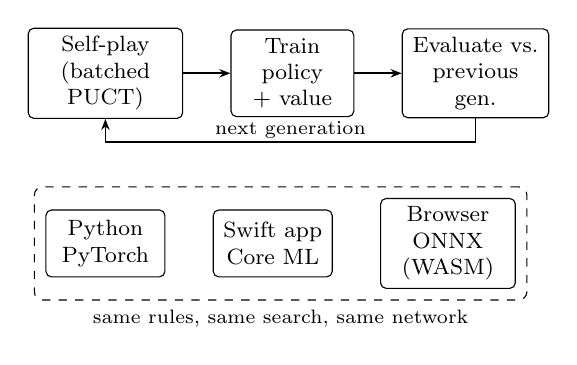
\begin{tikzpicture}[
    box/.style={draw, rounded corners=2pt, align=center, font=\footnotesize, minimum height=0.85cm, inner sep=3pt},
    arr/.style={-{Stealth[length=4pt]}, semithick},
    node distance=0.35cm and 0.6cm]
  \node[box, text width=1.75cm] (self) {Self-play\\(batched PUCT)};
  \node[box, text width=1.35cm, right=of self] (train) {Train\\policy + value};
  \node[box, text width=1.65cm, right=of train] (eval) {Evaluate vs.\\previous gen.};
  \draw[arr] (self) -- (train);
  \draw[arr] (train) -- (eval);
  \draw[arr] (eval.south) |- ++(0,-0.3) -| node[pos=0.25, above=1pt, font=\scriptsize, inner sep=0pt] {next generation} (self.south);
  \node[box, text width=1.3cm, below=1.15cm of self] (py) {Python\\PyTorch};
  \node[box, text width=1.3cm, right=of py] (sw) {Swift app\\Core ML};
  \node[box, text width=1.5cm, right=of sw] (js) {Browser\\ONNX (WASM)};
  \node[draw, dashed, rounded corners=3pt, fit=(py)(sw)(js), inner sep=4pt,
        label={[font=\scriptsize]below:same rules, same search, same network}] {};
\end{tikzpicture}
\caption{One training loop on a laptop CPU; the same rules, search and trained network run in three
runtimes. Chained Elo comes from the ``evaluate vs.\ previous generation'' step.}
\label{fig:pipeline}
\end{figure}

\paragraph{Game and representation.}
We play 9$\times$9 Go with simple ko, no suicide and Tromp--Taylor area scoring (komi 7.5); games end
after two passes or 162 moves. The network sees six planes: each side's stones now and one move ago, the
side to move, and a constant plane.

\paragraph{Network and search.}
A residual network \citep{he2016resnet} with \valNParams{} parameters (Table~\ref{tab:hyper}) outputs move
logits for the 81 points and pass, and a value in $[-1,1]$. Search is PUCT \citep{rosin2011puct} as in
AlphaZero, with one change from Leela Zero: an unvisited move is valued at the parent's value minus a
reduction that grows with the prior probability already explored (first-play urgency).

\paragraph{Self-play and training.}
Ten worker processes each play 16 games in lock step. Every simulation step evaluates one leaf per game in
a single network batch, which keeps a CPU busy without virtual loss or threads. Following KataGo
\citep{wu2019katago}, a quarter of moves receive a full search and become training samples; the rest get a
quarter of the simulations and only advance the game. The network trains with AdamW on a sliding window
of recent positions, with all eight board symmetries, on cross-entropy to the search's visit distribution
plus squared error to the game result. Each generation then plays the previous one in a
\valEvalGames{}-game match at \valEvalSims{} simulations a move; the summed Elo differences form the
chained Elo of the training log.

\begin{table}[t]
\centering
\small
% generated by figures_scripts/hyperparams_table.py
\begin{tabular}{@{}ll@{}}
\toprule
Setting & Value \\
\midrule
Board, komi, move cap & 9$\times$9, 7.5, 162 \\
Input planes & 6 \\
Residual blocks $\times$ channels & 4 $\times$ 48 \\
$c_{\mathrm{puct}}$, FPU reduction & 1.5, 0.25 \\
Dirichlet $\alpha$, $\varepsilon$ & 0.12, 0.25 \\
Sims: full / fast search & 160 / 40 \\
Full-search probability & 0.25 \\
Temperature-1 moves & 10 \\
Games / generation, workers & 160, 10 \\
Batch, learning rate (AdamW) & 256, 0.001 \\
Replay window (positions) & 250,000 \\
Chained eval: games, sims & 40, 32 \\
\bottomrule
\end{tabular}
\caption{Settings of the run, read from the training code and its saved configuration.}
\label{tab:hyper}
\end{table}

\paragraph{Hardware and budget.}
Everything ran on one Intel Core i9-9980HK (8 cores, 16 threads, no GPU). The run took \valNGens{}
generations of \valGamesPerGen{} games each (\valTotalGames{} games, about \valWallHours{} hours of wall-clock
time). That time is approximate: other software shared the machine, and one generation's self-play
took anywhere from \valSelfplayMin{} to \valSelfplayMax{} seconds. Figure~\ref{fig:loss} shows the losses.

\begin{figure}[t]
\centering
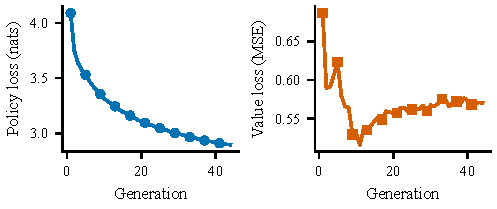
\includegraphics[width=\columnwidth]{figures/loss_curves.pdf}
\caption{Training losses fall steadily across generations: policy cross-entropy from
\valPolicyLossFirst{} to \valPolicyLossLast{} nats, and value MSE from \valValueLossFirst{} to
\valValueLossLast{}. One run.}
\label{fig:loss}
\end{figure}
\section{Evaluating a Small Self-Play Run}
\label{sec:evaluation}
\paragraph{Chained Elo and its noise.}
Let $p_g$ be the score of generation $g$ against $g-1$ in an $n$-game match. Chained Elo is
$E_g=\sum_{i\le g} 400\log_{10}\bigl(p_i/(1-p_i)\bigr)$, with $p_i$ clipped to $[0.02,0.98]$. Each term
has a standard error of about $\frac{400}{\ln 10}\cdot\frac{\sqrt{0.25/n}}{0.25}$ at $p=0.5$, which is
\valStepSE{} Elo for $n=\valEvalGames{}$. The errors are independent, so they add like a random walk: after
\valNGens{} generations the spread from noise alone is $\pm$\valWalkSD{} Elo (one standard deviation). Two
generations far apart can therefore be ranked in the wrong order even when every step is unbiased.
Section~\ref{sec:results} shows that noise alone does not explain our run.

\paragraph{Anchored matches.}
To measure progress without chaining, we play every fourth generation ($0,4,\dots,44$) against the next two
sampled generations and against the final generation \valNGens{}. This gives \valAnchoredPairs{} pairs of
\valEvalGames{} games (\valAnchoredGames{} games), each at \valAnchoredSims{} simulations a move, with
colors balanced and moves sampled in proportion to visits for the first six moves. Together with eleven
80-game checks played between release candidates, that gives \valHtoHGames{} games. We report the results
in two ways:
\begin{itemize}
  \item \emph{model-free}: each sampled generation's score against the final one, with 95\% Wilson intervals;
  \item a Bradley--Terry fit \citep{bradley1952rank} on all games on the Elo scale (generation~0 $=0$), with
        a weak Gaussian prior (s.d.\ 1000) to keep one-sided results finite, and 95\% bootstrap intervals
        from resampling games within each match.
\end{itemize}

\paragraph{Consecutive replay.}
To separate the effect of short matches from the effect of comparing adjacent generations, we replay the
consecutive pairs from generation~\valConsFrom{} onwards at the anchored settings (\valConsPairs{} pairs,
40 games each, \valAnchoredSims{} simulations).
\section{Results}
\label{sec:results}
\begin{figure*}[t]
\centering
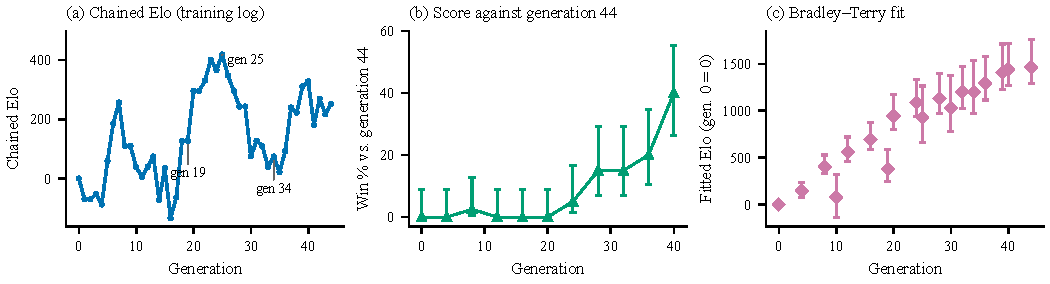
\includegraphics[width=\textwidth]{figures/elo_comparison.pdf}
\caption{Chained Elo says training stalled after generation~\valChainedPeakGen{}; anchored games say it kept
improving. (a)~Chained Elo from the training log (\valEvalGames{}-game matches against the previous
generation, \valEvalSims{} simulations). (b)~Score of every fourth generation against the final generation
\valNGens{} (\valEvalGames{} games each, \valAnchoredSims{} simulations), with 95\% Wilson intervals.
(c)~Bradley--Terry ratings fitted to all \valHtoHGames{} head-to-head games, with 95\% bootstrap intervals.
The model fits poorly at large rating gaps (see text), so read (c) as a ranking, not a scale.}
\label{fig:elo}
\end{figure*}

\paragraph{Chained Elo misranks the run.}
Figure~\ref{fig:elo}a shows the training log's chained Elo: a peak of \valChainedPeak{} at
generation~\valChainedPeakGen{}, a decline to \valChainedThirtyFour{} at generation~34, and \valChainedFinal{}
at the end. Every anchored measurement disagrees.
\begin{itemize}
  \item Head to head, generation~34 beats generation~25 in \valHTtfVsTf{} games and generation~19 in
        \valHTtfVsNt{}, and generation~\valNGens{} beats generation~34 in \valHFfVsTtf{}.
  \item Against the final generation, the scores of generations $0,4,\dots,40$ are \valAnchorScores{} wins
        out of \valEvalGames{}: flat at zero while the earlier networks are far weaker, then rising steadily
        from generation~24 (Figure~\ref{fig:elo}b), with no sign of the decline after generation~25.
  \item The Bradley--Terry ratings increase with generation apart from two less-constrained points (generations
        10 and 19, which appear only in a few long-range matches) (Figure~\ref{fig:elo}c).
\end{itemize}
The fit is approximate. Its Pearson $\chi^2$ is \valBTChiSq{} over \valBTMatches{} matches with
\valBTFree{} free ratings. Its residuals are systematic: in close pairs the newer network wins more often
than predicted, and in very lopsided pairs the weaker network still wins a few games, mostly through the
randomized opening. We therefore do not quote a total Elo gain from the fit.

\begin{figure}[t]
\centering
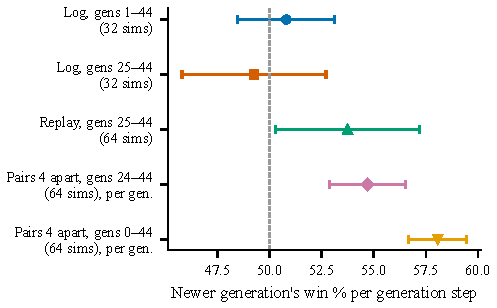
\includegraphics[width=\columnwidth]{figures/step_gain.pdf}
\caption{At 64 simulations, consecutive-generation matches agree with pairs four apart; the training log's
32-simulation matches measured almost no gain. Each row is the newer network's win rate for a single
generation step, with 95\% Wilson intervals; results for pairs four apart are converted to a single step
through the Elo scale. Compare rows over the same generations: gains are larger early in training.}
\label{fig:step}
\end{figure}

\paragraph{Why: noise contributes, but the cheap matches are the main cause.}
Pairs four generations apart give the newer network a pooled win rate of \valStepFourWr{}, or about
\valStepElo{} Elo per generation over the whole run. Over generations 24--44 alone, the rate is \valLateStepElo{}
Elo per generation, a per-generation win rate of \valLateStepWr{} (95\% interval \valLateStepWrLo{}--\valLateStepWrHi{}).
At that rate, chained Elo should have risen by about \valDropExpect{} from generation~25 to~34, with a
noise standard deviation of $3\times\valStepSE{}$ Elo. Instead it fell by \valInversion{}, \valDropZ{} standard
deviations from the expectation, so noise alone is an unlikely explanation.

The training log's matches were cheaper than our anchored ones: 32 simulations a move instead of 64.
Replaying the consecutive pairs from generation~\valConsFrom{} onwards at 64 simulations gives the newer network
\valConsWr{} of the games (95\% interval \valConsWrLo{}--\valConsWrHi{}), against \valConsWrLog{} for the same pairs
in the log. That is consistent with the \valLateStepWr{} implied by pairs four apart over the same generations
(Figure~\ref{fig:step}). Chained over generations 25 to 34, the replay gives \valReplayChain{} Elo, the correct direction
(the head-to-head result implies \valHtoHEloTtfTf{}), where the log gave $-$\valInversion{}. Over generations
\valConsFrom{}--\valNGens{} it gives \valReplayChainAll{}, where the log gave \valLogChainAll{}.

So comparing adjacent generations is not misleading in itself. In this run the per-generation matches were
too shallow to separate networks that, at deployment-like search depth, differ by a few dozen Elo, and summing
their noisy, compressed differences hid the trend. On any one pair the difference between the log and the
replay is within noise, so we cannot fully separate the effect of search depth from the play of chance with
one run. But every 64-simulation measurement in Figure~\ref{fig:step} points the same way.

\paragraph{External calibration.}
\label{sec:gnugo}
Against GNU~Go~3.8 at level \valGnuLevel{} (its weakest), with Chinese rules, komi 7.5 and
\texttt{-{}-capture-all-dead} so that our area scoring is fair to it, generation~\valNGens{} at \valGnuSims{}
simulations a move won \valGnuWins{} games, with a median losing margin of \valGnuMedianMargin{} points.
GNU~Go's own scoring named the same winner in \valGnuScoreAgree{} games. The internal gains above are real,
but in absolute terms the network remains far weaker than a classical engine at its weakest setting.

\paragraph{One engine, three runtimes.}
The rules are implemented three times: in Python for training, in Swift for the macOS app and in JavaScript
for the browser. All three agree exactly on the board, ko point, legal moves, score and input planes for
\valRuleCases{} positions taken from \valRuleGames{} random games, generated by the Python rules. The trained
network, exported to Core ML and to ONNX, matches PyTorch to within $\valCoreMLDiff\times10^{-6}$ and
$\valOnnxDiff\times10^{-6}$ on random inputs. On \valBenchPositions{} positions from a self-play game,
searched from scratch for \valBenchSims{} simulations each, the root visit counts were identical in
\valBenchIdentical{} positions on all three runtimes (Table~\ref{tab:platform}), so the app and the web page
make exactly the moves the trainer would.

\begin{table}[t]
\centering
\small
% generated by figures_scripts/platform_table.py
\begin{tabular}{@{}lrrrr@{}}
\toprule
Runtime & ms & sims/s & Same & Max $|\Delta|$ \\
\midrule
PyTorch & 974 & 411 & 15/15 & -- \\
Core ML & \textbf{534} & \textbf{750} & 15/15 & $5.5\times10^{-6}$ \\
ONNX (web) & 975 & 410 & 15/15 & $7.6\times10^{-6}$ \\
\bottomrule
\end{tabular}
\caption{The same search on three runtimes: PyTorch (Python trainer), Core ML (Swift app) and ONNX Runtime
Web (browser, WebAssembly). Columns: median time (ms) for a \valBenchSims{}-simulation search over
\valBenchPositions{} positions (best of three runs each, one leaf per network call, one CPU thread); positions
whose root visit counts equal PyTorch's exactly; largest network output difference from PyTorch.}
\label{tab:platform}
\end{table}
\section{Lessons for Small Runs}
\label{sec:lessons}
\paragraph{Evaluate against anchors, not only the predecessor.}
A protocol that fits a small budget and would have caught our false decline:
\begin{enumerate}
  \item Play evaluation games with at least the search depth you will deploy. Matches that are too
        shallow compress real differences toward a draw.
  \item Keep the consecutive-generation match for gating or monitoring if useful, but do not sum it into
        a strength curve. Every few generations, play the new network against a fixed set of anchors
        instead (an early generation, a mid-run generation and the most recent release).
  \item Report scores against the anchors with confidence intervals, and promote a network only when it
        beats the current release head to head.
\end{enumerate}
In our run, a single row of Figure~\ref{fig:elo}b, the score against one late anchor, already shows the trend
that chained Elo hid. It cost \valEvalGames{} games per sampled generation.

\paragraph{Engineering notes.}
Lock-step batched search keeps a CPU-only machine busy without threads. Playout-cap randomization makes
more games per hour \citep{wu2019katago}. Worker pools need timeouts. Python's \texttt{multiprocessing.Pool}
replaces a worker that dies but drops that worker's job, which once stalled our run for two hours on an
overloaded machine. Pool calls now time out and are retried on fresh workers. Running the rules in more
than one language paid for itself through shared test positions generated by the trainer.
\section{Limitations and Conclusion}
\paragraph{Limitations.}
This is one training run with one seed, on 9$\times$9 Go, with a small network. We do not know how often
chained Elo misleads in other runs, games or network sizes; the analysis of noise is general, but the size
of the effect of shallow evaluation may not be. We compared only 32 and 64 simulations a move, and replayed only
generations 24--44. On a single pair, the log and the replay differ by less than the noise, so the attribution
rests on the aggregate. Wall-clock times were measured on a
machine shared with other work. We played no games against humans, and the GNU~Go comparison used a single
setting.

\paragraph{Conclusion.}
On a small AlphaZero run, summing Elo from short matches between consecutive generations suggested a
stall and decline. Anchored head-to-head games showed steady improvement. The disagreement is too large to
be match noise alone. Replaying the same consecutive matches with more search per move recovered the
correct direction and agreed with the anchored games. For small runs we recommend evaluating at least at
deployment search depth, and tracking scores against a few fixed anchors, which costs little. The training pipeline, the evaluation data and the identical-across-runtimes engine are
released with the paper \TODO{add the anonymized artifact link for review; the public repository URL for camera-ready}.

\paragraph{Use of AI tools.}
The implementation (training pipeline, rules engines, apps, evaluation scripts and
benchmarks) was written with an AI coding assistant (Claude Code) under the authors' direction and checked by
the tests and parity checks in Section~\ref{sec:results}. The same assistant, with a paper-writing skill,
drafted text, wrote the scripts that generate figures, tables and in-text numbers from the logged data, and
formatted and verified references. The authors reviewed all content and are responsible for it.
\TODO{author: confirm this statement matches what you did, and edit as needed.}
\label{pw:mainend}

\begin{thebibliography}{18}
\providecommand{\natexlab}[1]{#1}

\bibitem[{Agarwal et~al.(2021)Agarwal, Schwarzer, Castro, Courville, and Bellemare}]{agarwal2021precipice}
Agarwal, R.; Schwarzer, M.; Castro, P.~S.; Courville, A.; and Bellemare, M.~G. 2021.
\newblock Deep Reinforcement Learning at the Edge of the Statistical Precipice.
\newblock In \emph{Advances in Neural Information Processing Systems 34}.

\bibitem[{Balduzzi et~al.(2018)Balduzzi, Tuyls, P{\'e}rolat, and Graepel}]{balduzzi2018reevaluating}
Balduzzi, D.; Tuyls, K.; P{\'e}rolat, J.; and Graepel, T. 2018.
\newblock Re-evaluating Evaluation.
\newblock In \emph{Advances in Neural Information Processing Systems 31}.

\bibitem[{Bradley and Terry(1952)}]{bradley1952rank}
Bradley, R.~A.; and Terry, M.~E. 1952.
\newblock Rank analysis of incomplete block designs: {I}. The method of paired comparisons.
\newblock \emph{Biometrika}, 39(3/4): 324--345.

\bibitem[{Braun(2026)}]{braun2026efficient}
Braun, B. 2026.
\newblock Engineering Efficient Self-Play Chess: Search, Replay, and Throughput Under Limited Compute.
\newblock arXiv:2609.37447.

\bibitem[{Coulom(2008)}]{coulom2008whr}
Coulom, R. 2008.
\newblock Whole-History Rating: A {Bayesian} Rating System for Players of Time-Varying Strength.
\newblock In \emph{Computers and Games}, volume 5131 of \emph{Lecture Notes in Computer Science}, 113--124. Springer.

\bibitem[{Czarnecki et~al.(2020)Czarnecki, Gidel, Tracey, Tuyls, Omidshafiei, Balduzzi, and Jaderberg}]{czarnecki2020spinning}
Czarnecki, W.~M.; Gidel, G.; Tracey, B.; Tuyls, K.; Omidshafiei, S.; Balduzzi, D.; and Jaderberg, M. 2020.
\newblock Real World Games Look Like Spinning Tops.
\newblock In \emph{Advances in Neural Information Processing Systems 33}.

\bibitem[{Elo(1978)}]{elo1978rating}
Elo, A.~E. 1978.
\newblock \emph{The Rating of Chessplayers, Past and Present}.
\newblock New York: Arco.

\bibitem[{He et~al.(2016)He, Zhang, Ren, and Sun}]{he2016resnet}
He, K.; Zhang, X.; Ren, S.; and Sun, J. 2016.
\newblock Deep Residual Learning for Image Recognition.
\newblock In \emph{IEEE Conference on Computer Vision and Pattern Recognition (CVPR)}, 770--778.

\bibitem[{Kocsis and Szepesv{\'a}ri(2006)}]{kocsis2006uct}
Kocsis, L.; and Szepesv{\'a}ri, C. 2006.
\newblock Bandit Based {Monte-Carlo} Planning.
\newblock In \emph{Machine Learning: ECML 2006}, volume 4212 of \emph{Lecture Notes in Computer Science}, 282--293. Springer.

\bibitem[{Lanctot et~al.(2023)Lanctot, Larson, Bachrach, Marris, Li, Bhoopchand, Anthony, Tanner, and Koop}]{lanctot2023vase}
Lanctot, M.; Larson, K.; Bachrach, Y.; Marris, L.; Li, Z.; Bhoopchand, A.; Anthony, T.; Tanner, B.; and Koop, A. 2023.
\newblock Evaluating Agents using Social Choice Theory.
\newblock arXiv:2312.03121.

\bibitem[{Lanctot et~al.(2019)Lanctot, Lockhart, Lespiau, Zambaldi, Upadhyay, P{\'e}rolat, Srinivasan, Timbers, Tuyls, Omidshafiei, Hennes, Morrill, Muller, Ewalds, Faulkner, Kram{\'a}r, De~Vylder, Saeta, Bradbury, Ding, Borgeaud, Lai, Schrittwieser, Anthony, Hughes, Danihelka, and Ryan-Davis}]{lanctot2019openspiel}
Lanctot, M.; Lockhart, E.; Lespiau, J.-B.; Zambaldi, V.; Upadhyay, S.; P{\'e}rolat, J.; Srinivasan, S.; Timbers, F.; Tuyls, K.; Omidshafiei, S.; Hennes, D.; Morrill, D.; Muller, P.; Ewalds, T.; Faulkner, R.; Kram{\'a}r, J.; De~Vylder, B.; Saeta, B.; Bradbury, J.; Ding, D.; Borgeaud, S.; Lai, M.; Schrittwieser, J.; Anthony, T.; Hughes, E.; Danihelka, I.; and Ryan-Davis, J. 2019.
\newblock {OpenSpiel}: A Framework for Reinforcement Learning in Games.
\newblock arXiv:1908.09453.

\bibitem[{Rosin(2011)}]{rosin2011puct}
Rosin, C.~D. 2011.
\newblock Multi-armed bandits with episode context.
\newblock \emph{Annals of Mathematics and Artificial Intelligence}, 61(3): 203--230.

\bibitem[{Sherwood, Aybar, and Kaplan(2026)}]{sherwood2026agents}
Sherwood, J.; Aybar, B.; and Kaplan, B. 2026.
\newblock Frontier Coding Agents Can Now Implement an {AlphaZero} Self-Play Machine Learning Pipeline For {Connect Four} That Performs Comparably to an External Solver.
\newblock arXiv:2604.25067.

\bibitem[{Silver et~al.(2016)Silver, Huang, Maddison, Guez, Sifre, van~den Driessche, Schrittwieser, Antonoglou, Panneershelvam, Lanctot, Dieleman, Grewe, Nham, Kalchbrenner, Sutskever, Lillicrap, Leach, Kavukcuoglu, Graepel, and Hassabis}]{silver2016alphago}
Silver, D.; Huang, A.; Maddison, C.~J.; Guez, A.; Sifre, L.; van~den Driessche, G.; Schrittwieser, J.; Antonoglou, I.; Panneershelvam, V.; Lanctot, M.; Dieleman, S.; Grewe, D.; Nham, J.; Kalchbrenner, N.; Sutskever, I.; Lillicrap, T.; Leach, M.; Kavukcuoglu, K.; Graepel, T.; and Hassabis, D. 2016.
\newblock Mastering the game of {Go} with deep neural networks and tree search.
\newblock \emph{Nature}, 529(7587): 484--489.

\bibitem[{Silver et~al.(2018)Silver, Hubert, Schrittwieser, Antonoglou, Lai, Guez, Lanctot, Sifre, Kumaran, Graepel, Lillicrap, Simonyan, and Hassabis}]{silver2018alphazero}
Silver, D.; Hubert, T.; Schrittwieser, J.; Antonoglou, I.; Lai, M.; Guez, A.; Lanctot, M.; Sifre, L.; Kumaran, D.; Graepel, T.; Lillicrap, T.; Simonyan, K.; and Hassabis, D. 2018.
\newblock A general reinforcement learning algorithm that masters chess, shogi, and {Go} through self-play.
\newblock \emph{Science}, 362(6419): 1140--1144.

\bibitem[{Silver et~al.(2017)Silver, Schrittwieser, Simonyan, Antonoglou, Huang, Guez, Hubert, Baker, Lai, Bolton, Chen, Lillicrap, Hui, Sifre, van~den Driessche, Graepel, and Hassabis}]{silver2017alphagozero}
Silver, D.; Schrittwieser, J.; Simonyan, K.; Antonoglou, I.; Huang, A.; Guez, A.; Hubert, T.; Baker, L.; Lai, M.; Bolton, A.; Chen, Y.; Lillicrap, T.; Hui, F.; Sifre, L.; van~den Driessche, G.; Graepel, T.; and Hassabis, D. 2017.
\newblock Mastering the game of {Go} without human knowledge.
\newblock \emph{Nature}, 550(7676): 354--359.

\bibitem[{Tian et~al.(2019)Tian, Ma, Gong, Sengupta, Chen, Pinkerton, and Zitnick}]{tian2019elf}
Tian, Y.; Ma, J.; Gong, Q.; Sengupta, S.; Chen, Z.; Pinkerton, J.; and Zitnick, L. 2019.
\newblock {ELF} {OpenGo}: an analysis and open reimplementation of {AlphaZero}.
\newblock In \emph{Proceedings of the 36th International Conference on Machine Learning}.

\bibitem[{Wu(2019)}]{wu2019katago}
Wu, D.~J. 2019.
\newblock Accelerating Self-Play Learning in {Go}.
\newblock arXiv:1902.10565.

\end{thebibliography}

\end{document}
